\documentclass{beamer}
\usepackage{ctex, hyperref}
\usepackage[T1]{fontenc}

% other packages
\usepackage{latexsym,amsmath,xcolor,multicol,booktabs,calligra}
\usepackage{graphicx,pstricks,listings,stackengine}

\author{Yajie Wu}
\title{The Least-Mean-Square(LMS)Algorithm}
\subtitle{Lecture note}
\institute{Shanghai University}
\date{2024年9月26日}
\usepackage{whu}

% defs
\def\cmd#1{\texttt{\color{red}\footnotesize $\backslash$#1}}
\def\env#1{\texttt{\color{blue}\footnotesize #1}}
\definecolor{deepblue}{rgb}{0,0,0.5}
\definecolor{deepred}{rgb}{0.6,0,0}
\definecolor{deepgreen}{rgb}{0,0.5,0}
\definecolor{halfgray}{gray}{0.55}

\lstset{
    basicstyle=\ttfamily\small,
    keywordstyle=\bfseries\color{deepblue},
    emphstyle=\ttfamily\color{deepred},    % Custom highlighting style
    stringstyle=\color{deepgreen},
    numbers=left,
    numberstyle=\small\color{halfgray},
    rulesepcolor=\color{red!20!green!20!blue!20},
    frame=shadowbox,
}


\begin{document}

\kaishu
\begin{frame}
    \titlepage
    \begin{figure}[htpb]
        \begin{center}
            
\includegraphics[width=0.2\linewidth]{pic/shu.png}
        \end{center}
    \end{figure}
\end{frame}

\begin{frame}
    \tableofcontents[sectionstyle=show,subsectionstyle=show/shaded/hide,subsubsectionstyle=show/shaded/hide]
\end{frame}


\section{Introduction}

\begin{frame}
    \begin{itemize}%[<+-| alert@+>] % 当然,除了alert,手动在里面插 \pause 也行
        \item  The least-mean-square (LMS) is a search algorithm in which a simplification of the gradient vector computation is made possible by appropriately modifying the objective function .  
        \item  The convergence characteristics of the LMS algorithm are examined in order to establish a range for the convergence factor
        that will guarantee stability. The convergence speed of the LMS is shown to be dependent on the eigenvalue spread of the
        input signal correlation matrix . 
        \item   The main features that attracted the use of the LMS algorithm are low computational complexity, proof of convergence in stationary environment,unbiased convergence in the mean to the Wiener solution, and stable behavior when implemented with finite-precision arithmetic. 
    \end{itemize}
\end{frame}


\section{The LMS Algorithm}

\subsection{basic problem}

\begin{frame}
    \begin{itemize}
        \item In Chap.2 , the optimal solution leads to the minimum mean-square error in estimating the reference signal d(k).
        \item The solution is given by
             \begin{equation}
            w_{o}=R^{-1}p
            \end{equation}
        where $R = E[x(k)x^{T}(k)]$ and $p = E[d(k)x(k)]$, assuming that d(k) and x(k) are jointly WSS.
        \item If good estimates of matrix $R$, denoted by $\hat{R}(k)$, and of vector $p$, denoted by $\hat{p}(k)$, are available, a steepest-descent-based algorithm can be used to search the Wiener solution of (1) as follows:
            \begin{equation*}
                w(k+1)= w(k) - \mu \hat{g}_{w}(k)
            \end{equation*}
            \begin{equation}
                \quad =w(k) + 2\mu (\hat{p}(k)-\hat{R}(k)w(k)) 
            \end{equation} 
        \item  for $k= 0,1,2,..., $where$\hat{g}_{w}(k) $represents an estimate of the gradient vector of the objective function with respect to the filter coefficients.
    \end{itemize}
\end{frame}

\begin{frame}
    \begin{itemize}
        \item One possible solution is to estimate the gradient vector by employing instantaneous estimates for R and p as follows:
       \begin{equation*}
        \hat{R}(k) = x(k)x^T(k)
       \end{equation*}
       \begin{equation}
        \hat{p}(k) = d(k)x(k)
       \end{equation}
       \item The resulting gradient estimate is given by 
       \begin{multline}
        \hat{g}_{w}(k)=-2d(k)x(k)+2x(k)x^T(k)w(k)\\
        =2x(k)(-d(k)+x^T(k)w(k))\\
        =-2e(k)x(k)\\
       \end{multline}
    \end{itemize}
\end{frame}

\begin{frame}
    \begin{itemize}
        \item Note that if the objective function is replaced by the instantaneous square error $e^2(k)$, instead of the MSE, the above gradient estimate represents the true gradient vector since
       \begin{multline}
       \frac{\partial e^2(k)}{\partial w}=\left[2e(k)\frac{\partial e(k)}{\partial w_0(k)} \ 2e(k)\frac{\partial e(k)}{\partial w_1(k)}\cdots 2e(k)\frac{\partial e(k)}{\partial w_N(k)}\right]^T\\
       =-2e(k)x(k)\\
       =\hat{g}_w(k)\\
       \end{multline}
       \item The resulting gradient-based algorithm is known as the least-mean-square (LMS) algorithm, whose updating equation is
       \begin{equation}
        w(k+1) = w(k) + 2\mu e(k)x(k)
       \end{equation}
       where the convergence factor μ should be chosen in a range to guarantee convergence. 
    \end{itemize}
\end{frame}

\subsection{LMS Algorithm}
\begin{frame}
    \begin{table}[h]
        \centering
        \begin{tabular}{c|c}
            \textbf{Algorithm 1} LMS algorithm  \\
            \hline
            Initialization\\
            $x(-1)=w(0)=[0 \ 0 \cdots 0]^T$\\
            Do for k $\geq$ 0 \\
            $e(k) = d(k)-x^T(k)w(k)$\\
            $w(k+1)=w(k)+2\mu e(k)x(k)$
        \end{tabular}
    \end{table}
\end{frame}

\begin{frame}{LMS algorithm}
    \begin{figure}[htbp]
        \centering
        \vspace{-0.0cm}
        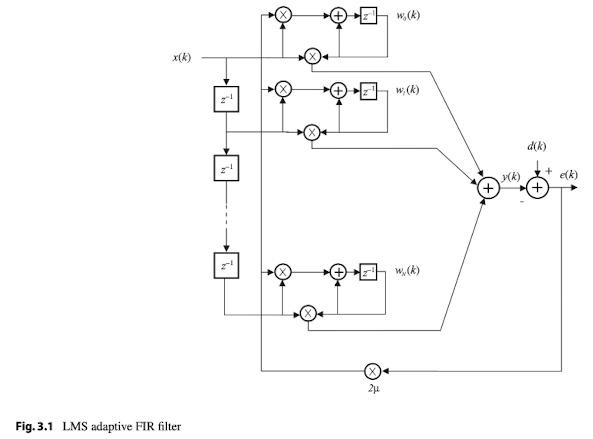
\includegraphics[scale=0.4]{pic/lms.png}
        \caption{1}
    \end{figure}
\end{frame}

\begin{frame}{code}
    \begin{figure}[htbp]
        \centering
        \vspace{-0.0cm}
        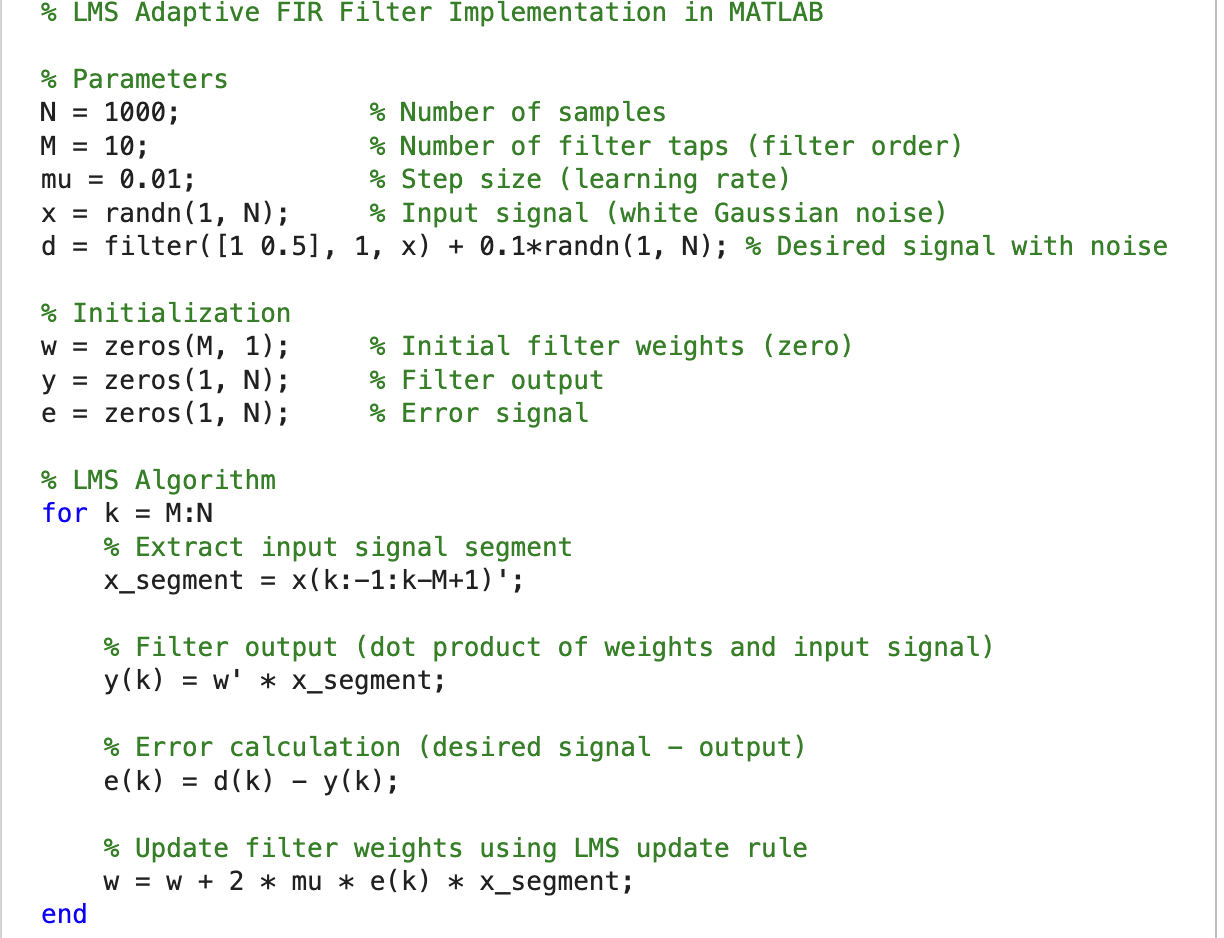
\includegraphics[scale=0.4]{pic/lms-code.png}
        \caption{2}
    \end{figure}
\end{frame}

\begin{frame}{simulation}
    \begin{figure}[htbp]
        \centering
        \vspace{-3.0cm}
        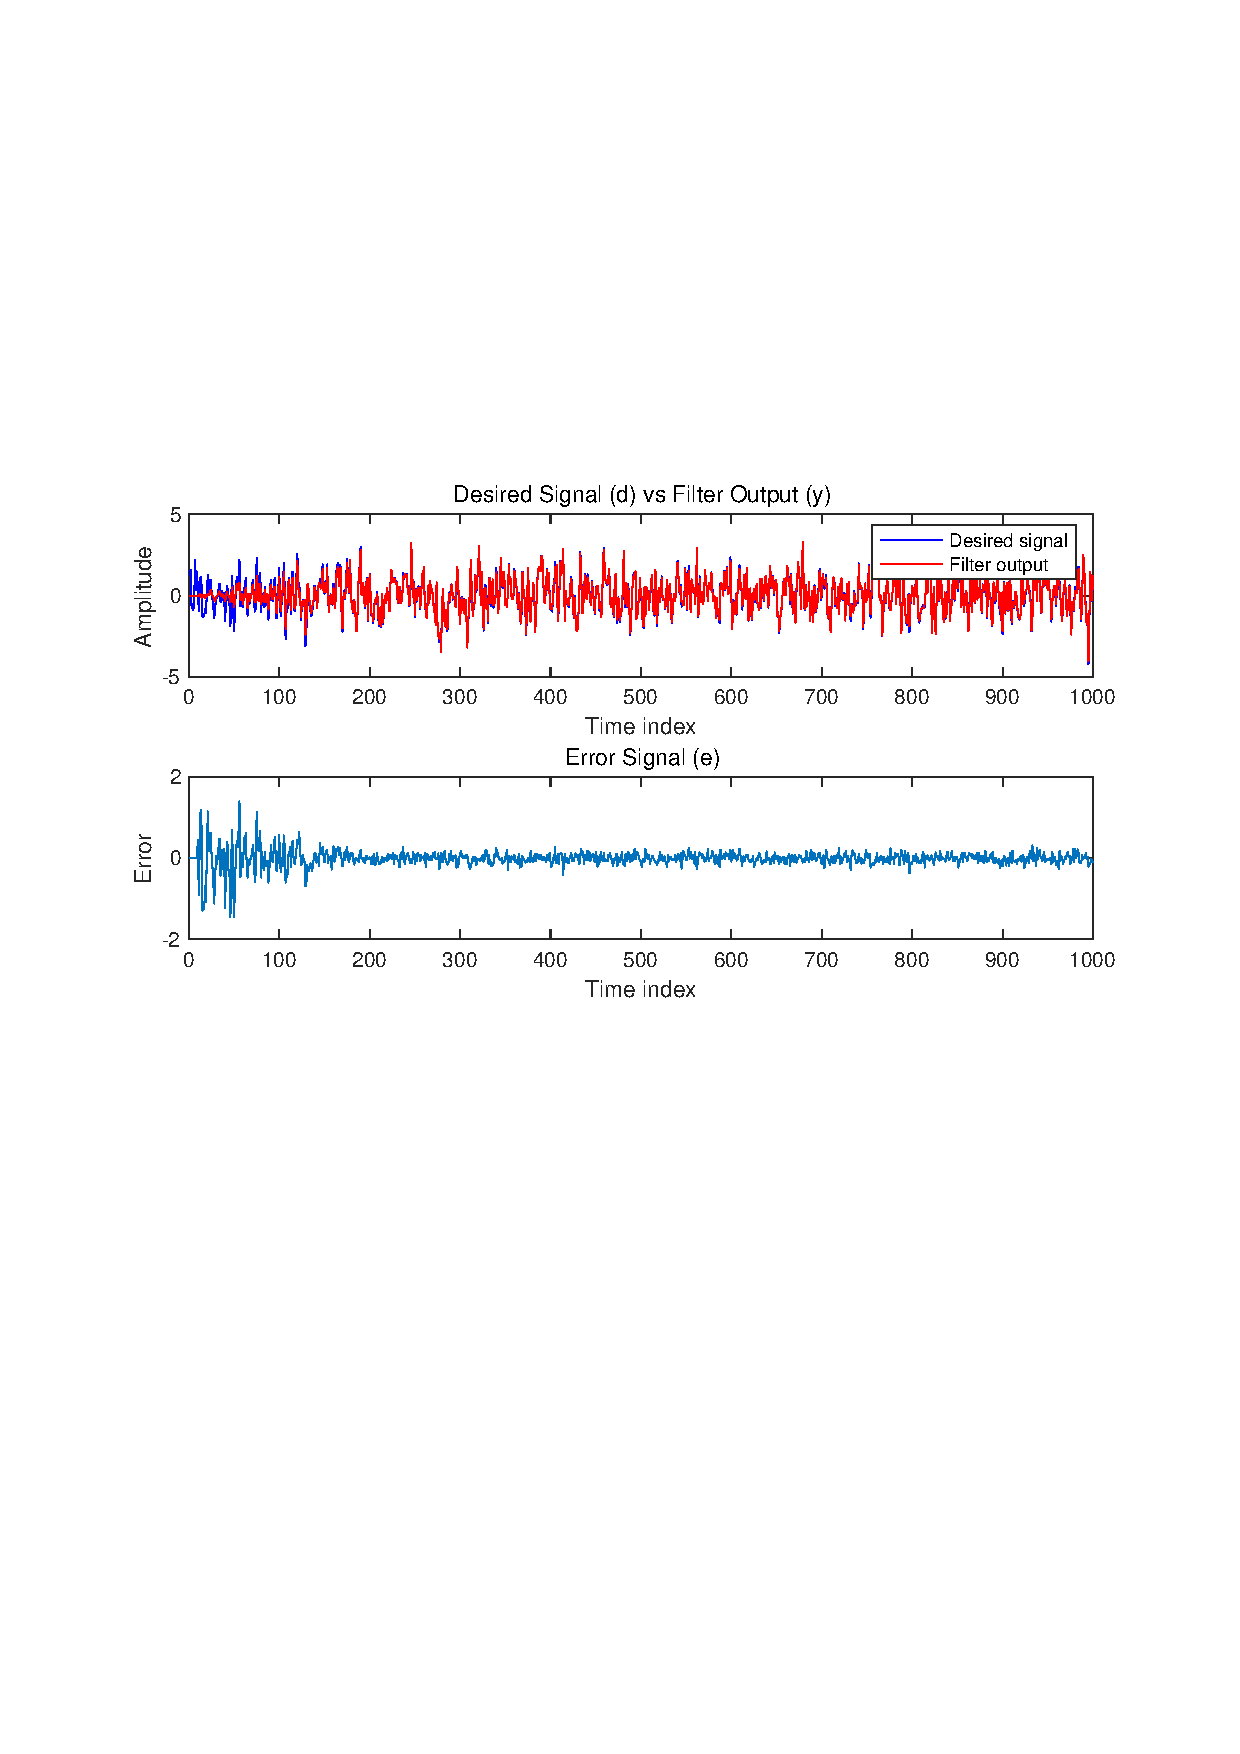
\includegraphics[scale=0.5]{pic/lms.pdf}
        \caption{3}
    \end{figure}
\end{frame}


\section{Some Properties of the LMS Algorithm}

\subsection{Gradient Behavior}

\begin{frame}{Gradient Behavior}
    \begin{itemize}
        \item he ideal gradient direction required to perform a search on the MSE surface for the optimum coefficient vector solution is
        \begin{equation*}
            g_w(k) = 2\{E[x(k)x^T(k)]w(k)-E(d(k)x(k))\}
        \end{equation*}
        \begin{equation}
        =2[Rw(k)-p]
        \end{equation}
        \item In the LMS algorithm, instantaneous estimates of R and p are used to determine the search direction, i.e.,
        \begin{equation}
            \hat{g}_w(k)=2[x(k)x^T(k)w(k)-d(k)x(k)]
        \end{equation}
    \end{itemize}
\end{frame}

\begin{frame}{Gradient Behavior}
    \begin{itemize}
        \item The LMS gradient direction has the tendency to approach the ideal gradient direction since for a fixed coefficient vector $ w $ .
        \begin{equation}
            E[\hat{g}_w(k)]=2{E[x(k)x^T(k)]w - E[d(k)x(k)]}=g_w
        \end{equation}
        \item vector $\hat{g}_w(k)$ can be interpreted as an unbiased estimate of $g_w$.
        \item In an ergodic environment, if, for a fixed $w$ vector, $\hat{g}_w(k)$ is calculated for a large number of inputs and reference signals, the average direction tends to $g_w$, i.e.,
        \begin{equation}
            \mathop{lim}\limits_{M \rightarrow \infty}\frac{1}{M}\sum\limits_{i=1}^{M}\hat{g}_w(k+i)\rightarrow g_w
        \end{equation}
    \end{itemize}
\end{frame}

\subsection{Convergence Behavior of the Coefficient Vector}

\begin{frame}{Convergence Behavior of the Coefficient Vector}
    \begin{itemize}
       \item Measurement white noise n(k) with zero mean and variance $\sigma^2_n$  is added to the output of the unknown system.
        \item The error in the adaptive filter coefficients as related to the ideal coefficient vector $w_o$, in each iteration, is described by the N + 1-length vector.
        \begin{equation}
            \Delta w(k)=w(k) - w_o
        \end{equation}
    \end{itemize}
\end{frame}

\begin{frame}{Convergence Behavior of the Coefficient Vector}
    \begin{itemize}
       \item LMS algorithm can alternatively be described by
        \begin{multline}
            \Delta w(k+1)=\Delta w(k) + 2\mu e(k)x(k)\\
                         =\Delta w(k) + 2\mu x(k)[x^T(k)w_o + n(k) - x^T(k)w(k)]\\
                         =\Delta w(k) + 2\mu x(k)[e_o(k) - x^T(k)\Delta w(k)]\\
                         =[I - 2\mu x(k)x^T(k)]\Delta w(k) + 2\mu e_o(k)x(k)
        \end{multline}
        $e_o(k)$ is the optimal output error given by 
        \begin{equation}
            e_o(k) = d(k) - w^T_o x(k) = w_o^T x(k) + n(k) -w_o^T x(k)=n(k)
        \end{equation}
    \end{itemize}
\end{frame}

\begin{frame}{Convergence Behavior of the Coefficient Vector}
    \begin{itemize}
       \item The expected error in the coefficient vector is then given by 
        \begin{multline}
            E[\Delta w(k+1)] = E\{[I - 2\mu x(k)x^T(k)]\Delta w(k)\} + 2\mu E[e_o(k)x(k)]
        \end{multline}
        \item If it is assumed that the elements of $x(k)$ are statistically independent of the elements of $w(k)$ and orthogonal to $e_o(k)$,(3.14) can be simplified as follows: 
        \begin{multline}
            E[\Delta w(k+1)] = \{I - 2\mu E[x(k)x^T(k)]\}E[\Delta w(k)]\\
                            = (I - 2\mu R)E[\Delta w(k)]\\
        \end{multline}
        \item The above expression leads to
        \begin{equation}
            E[\Delta w(k+1)] = (I - 2\mu R)^{k+1}E[\Delta w(0)]
        \end{equation}
    \end{itemize}
\end{frame}

\begin{frame}{Convergence Behavior of the Coefficient Vector}
    \begin{itemize}
       \item Equation (3.15) premultiplied by $Q^T$ , where Q is the unitary matrix that diagonalizes R through a similarity transformation,yields 
       \begin{multline}
        E[Q^T\Delta w(k+1)] = (I - 2\mu Q^TRQ)E[Q^T\Delta w(k)]\\
                           = E[\Delta w^{'}(k+1)]\\
                           = (I - 2\mu \Lambda)E[\Delta w^{'}(k)]\\
                           =\begin{bmatrix}
                            1-2\mu \lambda_0 & 0 & \cdots & 0 \\
                            0 & 1-2\mu \lambda_1 & \cdots & 0 \\
                            \vdots & \vdots & \ddots & \vdots \\
                            0 & 0 & \cdots &1-2\mu \lambda_N
                           \end{bmatrix}E[\Delta^{'}(k)]                  
        \end{multline}
         
        
    \end{itemize}
\end{frame}

\begin{frame}{Convergence Behavior of the Coefficient Vector}
    \begin{itemize}
       \item where $\Delta w^{'}(k + 1)= Q^T \Delta w(k + 1)$ is the rotated-coefficient-error vector. The applied rotation yielded an equation where the driving matrix is diagonal, making it easier to analyze the equation’s dynamic behavior. Alternatively, the above relation can be expressed as
       \begin{multline}
        E[Q^T\Delta w(k+1)] = (I - 2\mu \Lambda)^{k+1}E[\Delta w^{'}(0)]\\
                           ={\small\begin{bmatrix}
                            (1-2\mu \lambda_0)^{k+1} & 0 & \cdots & 0 \\
                            0 & (1-2\mu \lambda_1)^{k+1} & \cdots & 0 \\
                            \vdots & \vdots & \ddots & \vdots \\
                            0 & 0 & \cdots &(1-2\mu \lambda_N)^{k+1}
                           \end{bmatrix}E[\Delta^{'}(0)]}                  
        \end{multline} 
        
    \end{itemize}
\end{frame}

\begin{frame}{Convergence Behavior of the Coefficient Vector}
    \begin{itemize}
     \item This equation shows that in order to guarantee convergence of the coefficients in the mean, the convergence factor of the LMS algorithm must be chosen in the range 
     \begin{equation}
        0 < \mu < \frac{1}{\lambda_{max}}
     \end{equation}   
    \item The choice of $\mu$ as above explained ensures that the mean value of the coefficient vector approaches the optimum coefficient
    vector $w_o$. 
    \item It should be mentioned that if the matrix $R$ has a large eigenvalue spread, it is advisable to choose a value for $\mu$
    much smaller than the upper bound. 
    \end{itemize}
\end{frame}



\begin{frame}
    \begin{center}
        {\Huge\calligra Thanks!}
    \end{center}
\end{frame}

\end{document}
